

\documentclass[11pt,a4paper]{article} 
\setcounter{secnumdepth}{3}
\usepackage[T1]{fontenc}
\usepackage[utf8]{inputenc}
\usepackage{lmodern}
\usepackage{pdflscape}
\usepackage{lipsum}
\usepackage{graphicx}
\usepackage[margin=1.5in]{geometry}
\usepackage{caption}
\usepackage[font=footnotesize]{caption}
\usepackage{apacite}
\usepackage{color}
\usepackage{amsmath}
\usepackage{booktabs} 
\usepackage{xcolor}
\usepackage{float}
\usepackage{array}
\usepackage{setspace}
\usepackage{gensymb}
	\doublespacing
	
	\begin{document}
	
	
\section{Issues}


\begin{itemize}
\item How to justify using the addm for investigating context-dependence?
\item addm is already using relative value signals - our approach takes context dependence into account twice?
\item How to introduce the idea of normalised by max rule? 
\item probability approach: how to properly explain the axis rotation
\item probability approach: is the non-symmetric triangle an issue?
\item probability approach vs simulations parameter distribution
\end{itemize}

\newpage

\section{Introduction} \label{chap1intro}

short intro on types of context-dependence - most important examples?

While there is strong evidence that our decisions are profoundly affected by the decision context, how exactly the perceived subjective value of an option changes as a function of choice environment, is still a matter of debate within the literature. 

Over the past decades, several theoretical models of context-dependent valuation have been proposed. One of the earliest of these is Parducci's range-freguency theory (RFT; \citeNP{Parducci1963}, \citeyearNP{Parducci1965}), a highly influential theory in psychophysics, which offers an account of how objective stimuli get translated into subjective quantities. According to RFT, the perceived magnitude of the stimulus depends on two components, its range and rank value within the stimuli set. The range value of the stimulus reflects its position with respect to the highest and lowest stimuli in the set, whereas the rank value reflects its position within the ordered set of stimuli. RFT has proven to be a good explanatory framework for contexts effects observed in a range of domains, such as strategic decision making \cite{Vlaev2006a}, price judgments \cite{Niedrich2009}, and even pain perception \cite{Watkinson2013}.  


The range and rank principles have also been influential outside the RFT framework. For example, the effects of stimulus range on discrimination performance and magnitude judgments have long been the focus of perceptual psychology \cite{Lockhead1986}. More recently, range effects have been increasingly incorporated into models emerging from the interdisciplinary field of decision neuroscience. These models mostly focus on explaining patterns of neural activity during decision-making tasks in fMRI experiments. Given that neural firing rates are bounded from above due to biophysical constraints, it is a natural assumption that some sort of adaptive mechanism must take place to accommodate differences in the range of stimulus values that can be experienced in the real-world (e.g., \citeNP{Louie2013}; \citeNP{Padoa-Schioppa2009}; \citeNP{Soltani2012}; \citeNP{Rangel2012}).

%Value normalization in decision making: theory and evidence

The rank principle has also been successfully applied in a range of choice domains. For example, in an fMRI experiment where participants were shown pictures of monetary amounts they could win, \citeA{Mullett2013} have found that activity in certain brain regions reflected the current stimulus' rank position within the entire set of stimuli. In a socioeconomic context, several studies have shown that the rank position of one's income within their respective social reference group (e.g., workplace, neighbourhood), but not the absolute level of income, is a significant predictor of a series of health outcomes including mental health, self-reported happiness, and job satisfaction (e.g., \citeNP{Daly2015}; \citeNP{Boyce2010}; \citeNP{Clark2008}; \citeNP{Brown2008a}).

The range and rank principles are two distinct approaches to value normalisation, where the transformed values are required to fall between 0 and 1. These can be contrasted with simpler forms of normalisation, where the values are divided by the maximum value in the set, which serves as a natural reference point for a subjective valuation scale. In the context of a choice experiment, this maximum can be represented by the highest value in the current choice trial (the local maximum), or, equally, it can be the highest value experienced during the entire experiment (the global maximum), which is equivalent to simply normalising all values by a constant.

In this research project, our primary aim was to contrast these four different forms of context dependence (range, rank, local and global maximum normalisation) on the basis of their explanatory power. To this end, we designed two experiments, with two fundamentally different stimuli types. In both of these experiments, we presented participants with choice triplets, in the form of complex preferential stimuli in Experiment 1, and perceptual stimuli in Experiment 2. More importantly, the "objective value" of each of the three options in each trial could be quantified in both experiments, which allowed us to investigate how these four value transformation rules fare in predicting choice behaviour.

There is a wide range of choice models that can serve as a suitable framework to investigate context-dependence in value-based choice. In this research project, we chose to rely on the theoretical framework of a hugely influential cognitive model of choice, the drift diffusion model (ddm; \citeNP{Ratcliff1978b}) and one of its popular extensions, the attentional drift diffusion model (aDDM; \citeNP{Krajbich2010}; \citeNP{Krajbich2011}), which incorporates the role of eye-movements within the standard drift diffusion model. 

Using data from Experiment 1, we contrasted the four value transformation rules by fitting the four variants of the aDDM to the choice and RT data and compared the resulting likelihoods. Following this quantitative test, we also conducted a qualitative comparison of the four rules, by contrasting choice proportions from both experiments with our predictions from simulating out the four types of the ddm. The next section gives a brief overview of the ddm and its extension, the aDDM.



\subsection{The drift diffusion model} \label{chap1addmexplain}


How do people choose when facing multiple options? What happens exactly during the choice process, what is the cognitive mechanism underlying the comparison of the alternatives? These are the questions process models of choice seek to answer. In cognitive psychology, one particularly influential type of process models is the family of sequential sampling models. 

The overarching idea behind these models is that the evolution of preference in a given choice process is the result of noisy accumulation of evidence for each alternative throughout the decision process (hence the name “sequential sampling”), and a response is made when the accumulated evidence exceeds a certain threshold. Within the broader family of sequential sampling models, there is a wide variety of models depending on whether the evidence is accumulated separately and independently for each option and whether the threshold is defined to be absolute or relative (\citeNP{Forstmann2016}; \citeNP{Teodorescu2013}).

Of particular interest in psychology and cognitive neuroscience is a sequential sampling model that assumes a relative decision rule and a separate and independent accumulation process for each choice option under consideration. In discrete time, this is modelled as a random walk process, whereas in continuous time it can be characterised by a diffusion process. The latter form is called the ddm (e.g., \citeNP{Ratcliff1998a}; \citeNP{Ratcliff2008}), which is now the workhorse sequential sampling model in psychology and related fields. 

\begin{figure}[h]
\centering
\caption{Illustration of the evidence accumulation process with options A and
B.}
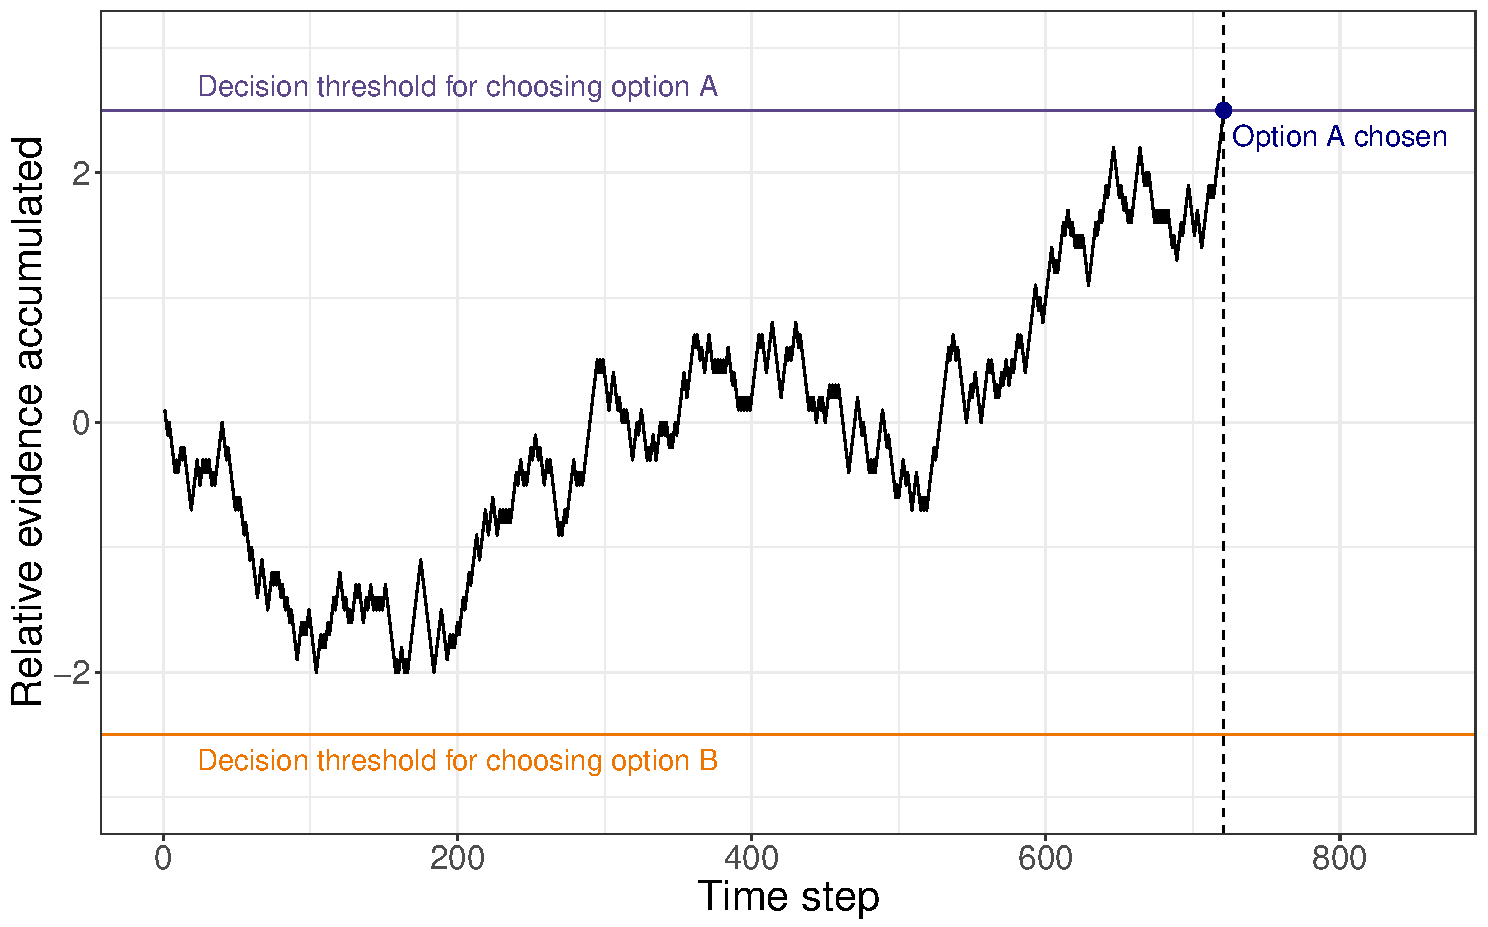
\includegraphics[width=0.8\textwidth]{c1_randomwalk.png}
\label{fig:randomwalk}
\end{figure}


In the drift diffusion framework, a key parameter of the model is the drift rate, which determines the average rate at which one of the thresholds are being approached during the choice process \cite{Voss2004a}. It also reflects the degree of similarity between the two options and thus can be seen as a measure of task difficulty: when the options are very similar and the task is difficult the process will have a low drift rate and therefore it will take longer to reach one of the thresholds. Conversely, when the options are easily discriminable and the choice is “easy”, the drift rate will be high and a threshold is reached faster. For a graphical illustration of the evidence accumulation process in the drift diffusion framework, see Figure \ref{fig:randomwalk}.

While the ddm in psychology was first used as a model of memory retrieval \cite{Ratcliff1978b}, it has since been applied in a wide range of choice task domains, including lexical decision making \cite{Ratcliff2004}, numerosity discrimination \cite{Leite2011} and emotional processing \cite{Mueller2016}. The popularity of the ddm in these choice tasks is due to a number of factors. 

First, and most importantly, it both predicts reaction time distributions and choice probabilities remarkably well (\citeNP{Ratcliff1999}; \citeNP{Forstmann2016}). Second, it has been shown that manipulations of the decision task (such as changing task difficulty, accuracy motivation and reward structure of the task) correspond to expected changes in model parameters (drift rate, threshold distance and the starting point of the accumulation process respectively), indicating that the model is successful in capturing the cognitive mechanism underlying choice processes \cite{Voss2004a}. Lastly, the model is inherently intuitive: it provides an elegant and plausible description of the evolution of preferences during the deliberation phase of decision making.

In addition to providing a psychologically plausible model of choice behaviour, the drift diffusion model has also been successfully applied in the field of cognitive neuroscience to explain both high- and low-level cognitive processes \cite{Forstmann2016}. Studies measuring decision-related neural activity in monkeys have found that over the course of a motion discrimination task, the firing rates of neurons in the lateral intraparetial cortex (LIP; an area in the brain responsible for attentional and decision-related processes, e.g. \citeNP{Shadlen2008}) exhibit a pattern which closely resembles to the accumulation of noisy evidence (e.g. \citeNP{Churchland2011}). In humans, studies using functional magnetic resonance imaging (fMRI) have identified distinct areas of the brain whose activation changes following value manipulations of model parameters (through changing the task design) in the ddm (for a review see \citeNP{Mulder2014}). 

Owing to the popularity of the ddm, several extensions of the model have been proposed. One notable example is the incorporation of attentional processes in binary and trinary value-based decisions, the attentional drift diffusion model (henceforth aDDM;  \citeNP{Krajbich2010}; \citeNP{Krajbich2011}). In the aDDM, visual fixations on one of the alternatives during the choice process alter the speed of evidence accumulation for the options. The mathematical formulation of the accumulation process in the trinary case with options left, center and right, when option left is fixated is as follows:

\begin{equation}
E_{t}^{left}=E_{t-1}^{left}+d\cdot r^{left}+\varepsilon_{t}^{left}
\end{equation}

\begin{equation}
E_{t}^{center}=E_{t-1}^{center}+\theta\cdot d\cdot r^{center}+\varepsilon_{t}^{center}
\end{equation}


\begin{equation}
E_{t}^{right}=E_{t-1}^{right}+\theta\cdot d\cdot r^{right}+\varepsilon_{t}^{right},
\end{equation}

where $E_{t}$ is the amount of evidence accumulated for a given option
(the value of the accumulator corresponding to an alternative) up
until time period $t$, $\theta$ is the penalty on the unattended
items (since $0<\theta<1$), $d$ is the rate of integration (a constant),
$r$ is the value of the given option and $\varepsilon$ is the noise
in the accumulation process. Therefore, for a given option, the total
amount of accumulated evidence in each time period is given by the
sum of the value of that accumulator in the previous time period,
the value of the option discounted by the penalty on the unattended
item (if it is not currently attended), and noise $\varepsilon\sim N(0,\sigma^{2})$.
The relative evidence accumulated for each option is defined as follows:

\begin{equation}
V_{t}^{left}=E_{t}^{left}-max(E_{t}^{center},E_{t}^{right})
\end{equation}

\begin{equation}
V_{t}^{center}=E_{t}^{center}-max(E_{t}^{left},E_{t}^{right})
\end{equation}


\begin{equation}
V_{t}^{right}=E_{t}^{right}-max(E_{t}^{left},E_{t}^{center})
\end{equation}

%As can be seen form the equations, the aDDM developed by Krajbich and Rangel \cite{Krajbich2011} implements a next to best decision rule: at any given time step, each item competes with the higher out of the other two. A choice is made when one of the relative evidence accumulators reach a given threshold (this is defined to be 1 in the specification given by Krajbich and Rangel). The free parameters in the model are \theta, d and \sigma^{2}. Figure \ref{fig:driftrates} illustrates an accumulation process in the aDDM framework. In general, the relative decision value for the fixated item increases, while it decreases for the unfixated items. The speed of the accumulation also depends on the value of the option. 

\begin{figure}
\centering
\caption{Illustration of the evidence accumulation process in the aDDM framework
($\mathit{\mathit{r^{left}=4,r^{center}=3,r^{right}=6,d=0.0002,}\theta=0.3,\sigma^{2}=0.001}$}
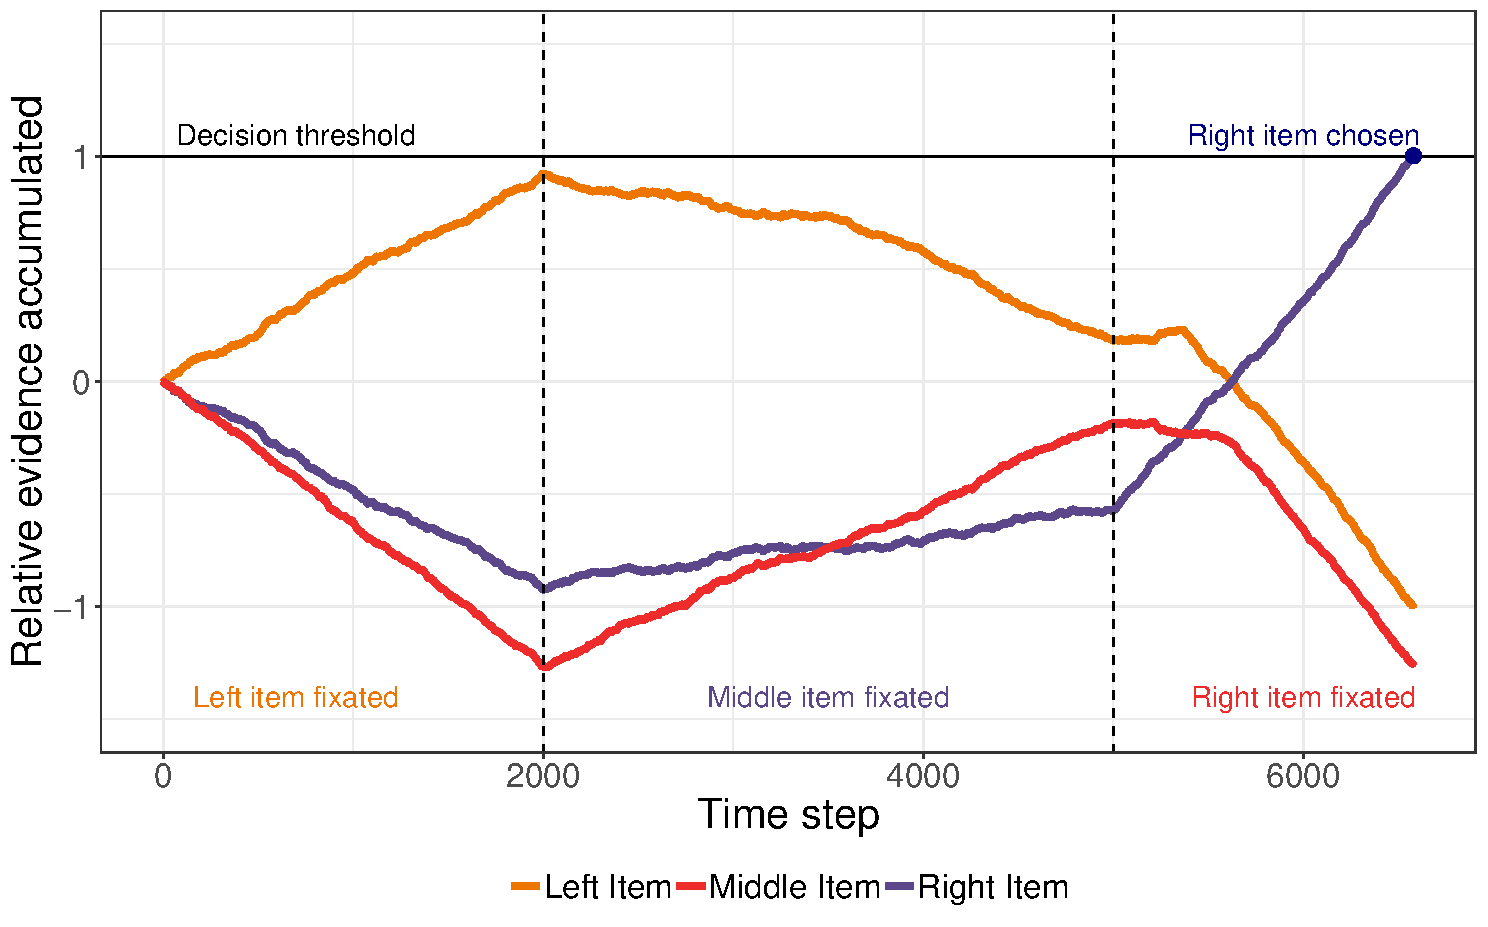
\includegraphics[width=0.8\textwidth]{c1_driftrates.png}
\label{fig:driftrates}
\end{figure}

The assumption that eye movements affect preference formation has been a subject of debate in the literature. In a preferential choice experiment by \citeNP{Shimojo2003}, they used pairs of faces used as stimuli, and found that were more likely to fixate on the item they ended up choosing, a phenomenon called the gaze bias, which has also been observed in other eye tracking experiments involving preferential choice (e.g. \citeNP{Armel2008}; \citeNP{Bird2012}). This effect tends to be especially pronounced towards the end of the decision: when retrospectively plotting how attention changes seconds before the choice was made, there is a much higher likelihood of the finally fixated item being the finally chosen one too (compared to the beginning of the trial). This is called the gaze cascade effect (e.g. \citeNP{Shimojo2003}; \citeNP{Glaholt2009}) or the late onset bias \citeNP{Mullett2016}. \citeA{Shimojo2003} argued that this effect is a result of a feedback loop between preference and visual orienting behaviour. 

According to their gaze cascade hypothesis, two effects, preferential looking (people are more likely to fixate on items they like) and the exposure effect (the longer people fixate on an item the stronger their preference will be for it) gradually reinforce each other, eventuating in the gaze cascade. Their experiments had shown that people are more likely to choose the face presented for longer only when fixating on the stimuli requires an eye movement (through lateral versus central presentation of the two stimuli), therefore they concluded that eye movements have a causal role in preference formation. However, using the same experiment with an improved design (larger sample size and accounting for potential masking effects in the central condition), \citeNP{Bird2012} found that same pattern of increased preference for the item presented for longer in the central condition, posing a serious challenge to the assumption that visual fixations have a causal effect on choice.


While the causal role of fixations in choice behaviour is not critical in the aDDM framework, the model can accommodate both the gaze bias and gaze cascade effect. First, fixating on one item for longer means that the amount of relative evidence accumulated in favour of this item will be larger, therefore it is more likely to be finally chosen (gaze bias effect). Second, because evidence accumulation is faster when an item is being fixated, it is more likely that the item's relative evidence accumulator reaches the threshold during a fixation on that item (gaze cascade effect). Comparisons of aDDM predictions and actual eye-tracking data have shown that the aDDM provides a remarkably good fit to the fixation, reaction time and choice data (\citeNP{Krajbich2010}; \citeNP{Krajbich2011}).

When fitting the aDDM to actual data, the value of the options (and hence the drift rate) is usually given by item ratings given by participants in a ratings task that precedes the choice task. This rating is assumed to reflect the “objective value” of an option, evaluated independently of the other options available. However, this need not be the case. In fact, there are ample evidence in the decision making literature suggesting that choice and valuation are inherently context-dependent. The idea that values and quantities have subjective mental representations that might considerably differ from their absolute magnitudes is the central tenet of psychophysics, which is concerned with the subjective magnitude estimation of physical stimuli \cite{Stevens1957}. Using a wide range of decision domains from perceptual judgment to value-based decisions, several studies have demonstrated that this subjective magnitude representation reflects the current or a recently experienced choice context. 


explain the parameters and that the drift diffusion model is the same without theta

explain that our model variants relate to how the options are encoded in the brain, and is not about how they are compared - that is unchanged compared to the original model


\section{Overview of Experiment 1 and 2}

In the following experiments, our goal was to capture the idea of context sensitivity within a the drift diffusion model framework. Using the model's terminology described in section \ref{chap1addmexplain}, we chose to incorporate these four forms of context-sensitivity through the the drift rate parameter (\textit{r} in the accumulation equation), and tested the four model variations' explanatory power.

Experiment 1 was a preferential choice experiment, where participants were presented with choice triplets created from movie posters. We also recorded their eye movements during choice. In a separate rating task that preceded the choice task, we obtained independent preference ratings from each participant on a set of 100 movies. Using these ratings as inputs to the value transformation rules, we investigated how the choice context affects the preferences over the options. In Experiment 2, we were interested in the same question, but we used perceptual stimuli, in the form of rapidly updating sequences of numbers drawn from a normal distribution with a fixed mean (taken from \citeNP{Tsetsos2012a}). Analogously, we used these fixed means as inputs to the value transformation rules.


For a thorough investigation of the explanatory power of the four value transformation rules, we used two fundamentally different approaches, a quantitative and qualitative approach. First, using data on eye movements during choice from Experiment 1, we obtained the best fitting set of aDDM model parameters for each valuation rule an participant, and compared the resulting likelihoods across the four value transformation rules. In order to obtain these best fitting parameters, we used two alternative methods to estimate the choice probabilities: a traditional simulations-based method, and a novel probability distribution method, which circumvents the problem arising from simulating out a stochastic model. Second, using a ddm simulations approach, we compared the choice proportion predictions for each value transformation rule with the results from Experiment 1 and 2, which served as a further qualitative test of the explanatory performance of each rule. 

Results from the model fitting approach suggest that subjective valuation mostly depends on the absolute value of the choice options, and to a lesser extent, also reflects  relative value sensitivity, a finding which was supported by the results from the qualitative comparison as well. We discuss these results in light of findings from neuroeconomic studies investigating the neural correlates of value-based choice.

\section{Subjective Transformation Rules} \label{chap1subjtrexplained}

We considered the four value transformation rules detailed in section \ref{chap1intro}: the range, rank, local maximum, and global maximum rule. Each rule takes in three "objective values" $x_1, x_2, x_3$  (these are the independent preference ratings for each movie in Experiment 1, and the mean of each distribution from which the rapidly updating sequence of numbers are drawn in Experiment 2), and transforms these into normalised "subjective values" (required to fall between 0 and 1). 

 \textbf{Range Rule.} The range value reflects the stimulus' perceived distance from the stimulus with the lowest value as a proportion of the overall distance between the highest and lowest valued stimulus in the stimuli set. It captures the idea that valuation is sensitive to the highest and lowest value encountered (or, equivalently, to the overall range of values) in a given choice set. Formally, this can be described by the following equation:
 
\begin{equation}
Range_{i}=\frac{x_i - min(x_1,x_2,x_3)}{max(x_1,x_2,x_3)-min(x_1,x_2,x_3)}
\label{eq:range}
\end{equation}
 Note that the items with the lowest and highest original values are always assigned 0 and 1 respectively, while the middle item's value can vary between 0 and 1.
 
 
 \textbf{Rank Rule.} The rank rule also follows from RFT, and reflects the “frequency” of the stimuli, which can be translated as its ranked ordinal position in the choice set. The rank rule reflects a somewhat simpler mechanism of valuation, whereby the subjective value of an item is solely determined by the number of items with lower or higher values in the choice set, and the extent of the difference between item values does not matter. Formally, given an ordered set of three stimuli $x_1, x_2, x_3$ , the rank value of a stimuli is given by
 
\begin{equation}
Rank_{i}=\frac{i-1}{n-1}
\label{eq:rank}
\end{equation}

Note that according to the rank rule, the three subjective values assigned to the items with the lowest, middle and highest value are always 0, 0.5 and 1, respectively.

\textbf{Local Maximum Rule.} The local maximum rule generates subjective value representations by dividing each stimuli's value by the highest value encountered on that trial, and in this way it corresponds to the normalised version of the raw ratings used in \citeA{Krajbich2011}. This reflects a bias towards the most rewarding, and hence potentially most salient option at the time of the choice. Formally, the subjective value of a stimuli according to the local maximum rule is given by

\begin{equation}
Local max_{i}=\frac{x_i}{max(x_1,x_2,x_3)}
\label{eq:locmax}
\end{equation}

Note that the stimuli with the highest value always assigned a subjective value of 1, while the other two values can vary between 0 and 1 (exclusive).

\textbf{Global Maximum Rule.} The global maximum rule is identical to the Local Maximum Rule, except that item values are normalised using the highest value encountered in the whole of the experiment (and not just on that trial). This means that all values are normalised by the same constant, therefore, the global maximum rule is equivalent to the original version of the aDDM, where they used the raw ratings participants gave in the preference rating task. Formally, in an experiment where the items that can be encountered are $x_1, x_2, ..., x_n$, the subjective value of a stimuli according to the global maximum rule is given by

\begin{equation}
Globalmax_{i}=\frac{x_i}{max(x_1,x_2,...,x_n)}
\label{eq:globmax}
\end{equation}

Note that when an item in the current trial has the highest value in the whole of the experiment this rule is equivalent to the local maximum rule, otherwise the values can vary between 0 and 1 (exclusive). 

\section{Choice Set Manipulations} \label{chap1choicesetman}

After identifying the four subjective transformation rules, the next step was to find a set of choice set manipulations for which these transformation rules (applied within an aDDM or ddm framework) derive different predictions about choice behaviour. Each of these manipulations represents some modification of the three options' objective values based on a certain rule (e.g. doubling each value, or adding a constant to each of them). This allowed us to assess the explanatory power of each value transformation rule by contrasting their respective choice predictions with the choice proportions derived from the data. The key idea is that the four transformation rules differ in their predictions about the effect of these choice set manipulations, which allowed us to assess the empirical performance of each subjective transformation rule.

Based on a series a simulations, we chose to investigate the effect of the following four distinct choice set manipulations: adding the same constant to each of the three values, multiplying each value by a constant, and having a distant or a close second, and third value. Figure \ref{fig:choicesetmanip} shows the subjective values (these are required to fall between 0 and 1) derived from each transformation, assuming a value scale from 1 to 7. The orange dots are the original values, while the purple dots show the values after the transformation (for example, in the case of adding a constant, the original value set is 1,2,4, while the transformed values are 4,5,7).

\begin{figure}
\captionsetup{justification=centering}
\centering
\caption{Subjective values by choice set manipulation and value transformation rule. The four columns show each choice set manipulation, while the rows correspond to the four subjective transformation rules.}
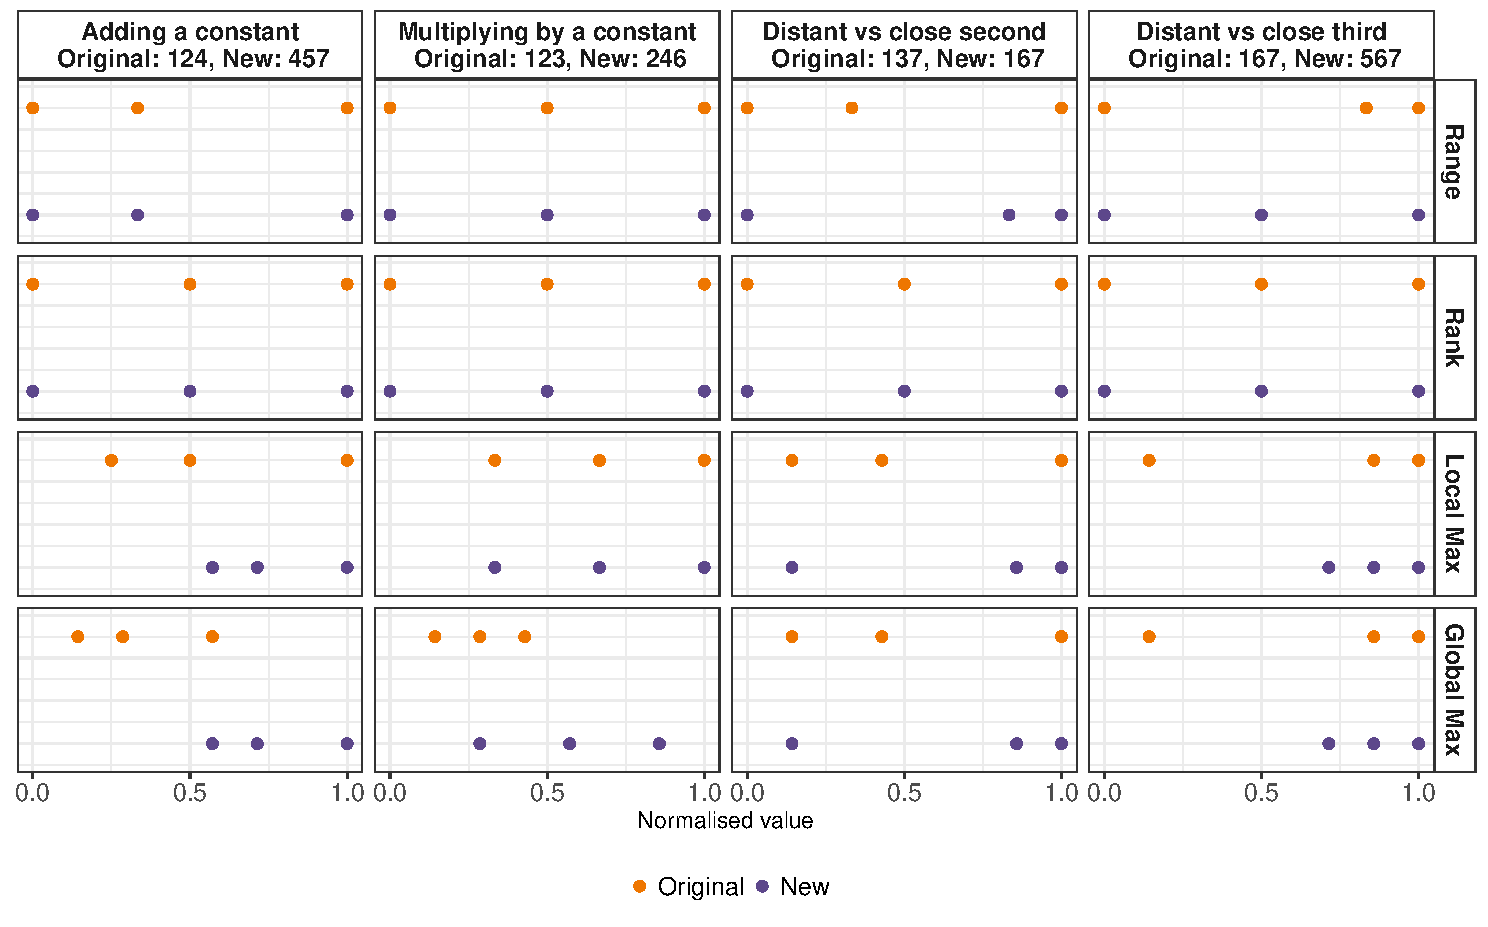
\includegraphics[width=1\textwidth]{explain.jpeg}
\label{fig:choicesetmanip}
\end{figure}

Our original plan was to present participants with these seven distinct choice sets (124, 457, 123, 246, 137, 167, 567) to maximise the discriminatory power of our experiments. However, due to an experimenter error, in Experiment 1, the displayed choice options were quasi-random, resulting in 84 unique choice sets instead of the originally planned seven. We nevertheless proceeded with fitting the aDDM to the data from Experiment 1, and had enough data for the relevant seven choice sets to conduct a qualitative comparison of choice behaviour in Experiment 1 and 2.


\section{Experiment 1}

\subsection{Method} \label{chap1exp1method}

Experiment 1 was a preferential choice experiment, where participant's eye movements were recorded during choice. Based on previous eye-tracking studies, we decided in advance that a sample of 50 participants should provide enough statistical power for our purposes. To reach this sample size, we recruited sixty participants overall, out of which ten participants could not be eye-tracked. Participants were recruited through the University of Warwick's Research Participation System and were paid £7.00 for taking part in the experiment. We did not record data on participants' gender, as we did not expect it to affect the results. Ethical approval was obtained from the Department of Psychology, University of Warwick.

The experiment consisted of two parts. First, participants who signed up for the study were required to complete an online questionnaire, where they had to rate 110 movies on a scale from 1 to 7, based on how much they liked the given movie (1 and 7 being not at all and very much so, respectively). We also asked them whether they have seen the movies before. The task began with 10 test trials (these were always the same movies), so that participants could familiarise themselves with the task. Then, they were informed that the actual task is about to start. During the main task, participants were presented with the 100 movies in a randomised order and we instructed them to try to use the whole range of the scale (as the second part of the experiment relied on these ratings and could not be run without at least one movie for each rating). Some participants failed to do this, and so they were asked again to complete this task before coming to the lab for the second part of the experiment. Figure \ref{fig:ratingstask} shows an example trial from this task, which took about 15 minutes on average. 

\begin{figure}
\captionsetup{justification=centering}
\centering
\caption{Example rating task from the first part of Experiment 1. }
\includegraphics[width=0.7\textwidth]{ratingstask.png}
\label{fig:ratingstask}
\end{figure}

Those who completed the first part were invited to the lab for the second part of the study. In the second part, participants were presented with 100 trinary sets of the pre-rated movies, and were asked to pick the one they liked the most on each trial by pressing the corresponding keyboard key (left, down, right arrow), while their eye movements were recorded at 500 Hz using an EyeLink 1000 (SR Research). The eye tracker was calibrated after every 25 choices (so four times overall over the course of the experiment), and each trial began after participants fixated on a centrally presented fixation cross for 500 ms. Figure \ref{fig:exp1_movieschoice} shows an example trial from the second part of this experiment.

\begin{figure}
\captionsetup{justification=centering}
\centering
\caption{Example choice task from the second part of Experiment 1. }
\includegraphics[width=0.7\textwidth]{exp1_movieschoice.jpg}
\label{fig:exp1_movieschoice}
\end{figure}



\subsection{Stimuli}

We chose 110 movies that received the most votes in 10 distinct genres (adventure, comedy, drama, family, fantasy, history, mystery, romance, sci-fi, thriller) on IMDb as of March, 2016. In the first part of the experiment, the first ten trials were practice trials (one movie from each genre), which aimed to give participants an idea about the range and type of movies they will be asked to rate. 

In the second part of the study, the displayed trinary sets were originally generated based on the participant's ratings to reflect the choice set manipulations. However, as mentioned above, the choice sets displayed during the experiment were quasi-random, due to the incorrect numbering of the 110 stimuli pictures (however, each number still corresponded to a unique movie). This resulted in 84 unique trinary choice sets, as opposed to the originally planned seven. 

In order to avoid the same set of movies appearing again, the display was generated to ensure that all the stimuli with a given rating gets used before any repetition occurs. We tried to vary the stimuli appearing as much as we could, but since some of the participants gave very uneven ratings (e.g., gave a rating of 1 to only one movie), in some cases repetition was inevitable. 

Given that our main aim was to fit each value transformation variant of the aDDM to the data, we decided it was worth proceeding with the analysis with the current dataset (even though the data now contained considerably fewer trials that could help us distinguish between the four value transformation rules). 

\subsection{Exclusion criteria}

As mentioned in section  \ref{chap1exp1method}, we had usable eye-tracking data from 50 participants. For a few participants, the calibration quality was not satisfactory in some parts of the experiment, and therefore we excluded these trials (account for about 2.5\% of all fixations). We also excluded the first three trials (as participants were getting used to using the keyboard at this stage), and each trial right after a calibration. We excluded fixations that outside the three areas of interest and trials in the upper 1\% of the RT distribution. Finally, we only kept trials where all three of the choice items were fixated at least once. 


\section{Fitting the aDDM}

Using data from Experiment 1, we wished to compare the fit of the four value transformation rules within the aDDM framework, on the basis of their respective likelihoods. As described in section \ref{chap1addmexplain}, there are three parameters in the aDDM: $\theta$, the penalty on the unattended item, $\sigma$, the noise parameter, and \textit{d}, the speed of integration. Our primary aim was to find the best fitting parameter set and the corresponding likelihood value for each participant and transformation rule (of which there 200, given 50 participants and four subjective value transformation rules) to determine which model variant fits best for each participant. Since the aDDM does not have a closed-form solution, we used two methods to obtain model predictions: a simulations and a probability distribution approach to derive choice probability and RT predictions for each model variant.

To incorporate the information on attention during choice, we first transformed the eye movements data into a form that can be processed by both aDDM implementations. More specifically, we divided each trial into 200 ms bins, where each bin was one step in the evidence accumulation process assumed by aDDM. The fixated item in a bin was sampled probabilistically based on the proportion of time spent on fixating on a given item in each bin. For example, if in one bin, 50 ms was spent on fixating on item 1, and 150 ms was spent on fixating on item 2, then in the simulations item 1 had 25\% while item 2 had 75\% chance of being chosen as the fixated item in that bin. 

We used the transformed ratings for fitting each of the four variants of the model. However, the wide variety of value triplets displayed in Experiment 1 (which was unintended) posed a question about how to derive the range transformed values in case there were two or three identical values in the choice set (it is straightforward in the case of the two maximum rules and the rank rule). We decided to code the transformed range values as 1 if all values were identical. If there were two equal values in a triplet, they were either coded as 1 or 0 (depending on whether the third value is lower or higher than the two identical ones, respectively). 

\subsection{Simulations method}

To obtain the likelihood of the data for each model variant, we first used a simulations method. Specifically, we simulated out each trial 100,000 times for all participants, and calculated the probability that the eventually chosen item was selected in the correct time bin. Note that there are two sources of variation in these simulations: the inherent noise in the accumulation process (captured by $\sigma$), and the non-deterministic fixation pattern arising from the transformation of the fixation data into time bins.

To find the best fitting parameter sets, we started off with a grid search with the following values: $\theta=\{0.2, 0.45, 0.6, 0.85, 1\}$, $\sigma=\{0.1, 0.14, 0.2, 0.28, 0.4\}$, $\textit{d}=\{0.1, 0.17, 0.31, 0.56, 1\}$, $5x5x5 = 125$ parameter sets overall, for each participant and value transformation rule. These values were chosen to make sure that most participants' best fitting values (from the values in the grid) fell in the middle of the value range. This was done to ensure that in the optimization process, the algorithm does not have to move considerable lengths in the parameter space to find the best fitting parameter set.

Upon obtaining the best fitting parameter set from the grid, we started a Nelder-Mead optimization algorithm using these sets as starting points for each participant and transformation rule. This was repeated once more using the results from the first Nelder-Mead optimization process as a starting point, to increase the probability that we find the parameter set that produces the highest likelihood of producing the data. For the overwhelming majority of participants and transformation rules, running the second Nelder-Mead did not improve the likelihood substantially.

We initially used 100,000 simulations to lessen the effect of noise (an inherent feature of the aDDM) and obtain reliable estimates. However, an unanticipated effect of having such a high number of simulations was that trials that were not well predicted by the model ended up having a big effect on the Nelder-Mead process, indicating a non-smooth likelihood surface. For example, having just one simulation out of 100,000 that predicts a given trial's data can have a dramatic effect on the likelihoods (going from minus infinity to a potentially very high likelihood, depending on the predicted probability of the rest of the trials), causing the Nelder-Mead process to get stuck at this point. The Nelder-Mead method was initially developed for deterministic models, and it has been demonstrated that substantial noise in the underlying model can lead to false convergence (e.g., \citeNP{Chang2012}; \citeNP{BartonIvey1991}). To alleviate these concerns about the validity of the simulations method, we decided to compare the results from the simulations with those obtained from an alternative, deterministic implementation of the aDDM.


\subsection{Probability distribution method}

To circumvent the problem of the non-smooth likelihood surface, we utilised an alternative method that is free of stochasticity. Specifically, we calculated how the probability distribution over the relative evidence states ($E_{1}-E_{2}$ and $E_{1}-E_{3}$ from Equation x in section \ref{chap1addmexplain}) change as a function of time and the model parameters. This way, we could directly derive the the choice probability for each trial in our data.

In order to restrict the are of finished evidence states (corresponding to combinations of $E_{1}$, $E_{2}$ and $E_{3}$ where the threshold had been reached, and one of the options had been chosen) to a bounded area in the relative evidence space, we chose to analyse a rule where the process is terminated when the difference between the best option and the average of the other two reaches the threshold (see Figure \ref{fig:rulesfinished}), as opposed to the next best rule employed by \citeauthor{Krajbich2011}. However, we did not expect this modification to have a substantial effect on our results, since previous research had shown that the two rules yield very similar predictions (see the Appendix in \citeauthor{Krajbich2011}).

\begin{figure}
\captionsetup{justification=centering}
\centering
\caption{The finished evidence states with Next Best and Average of second and third termination rules.}
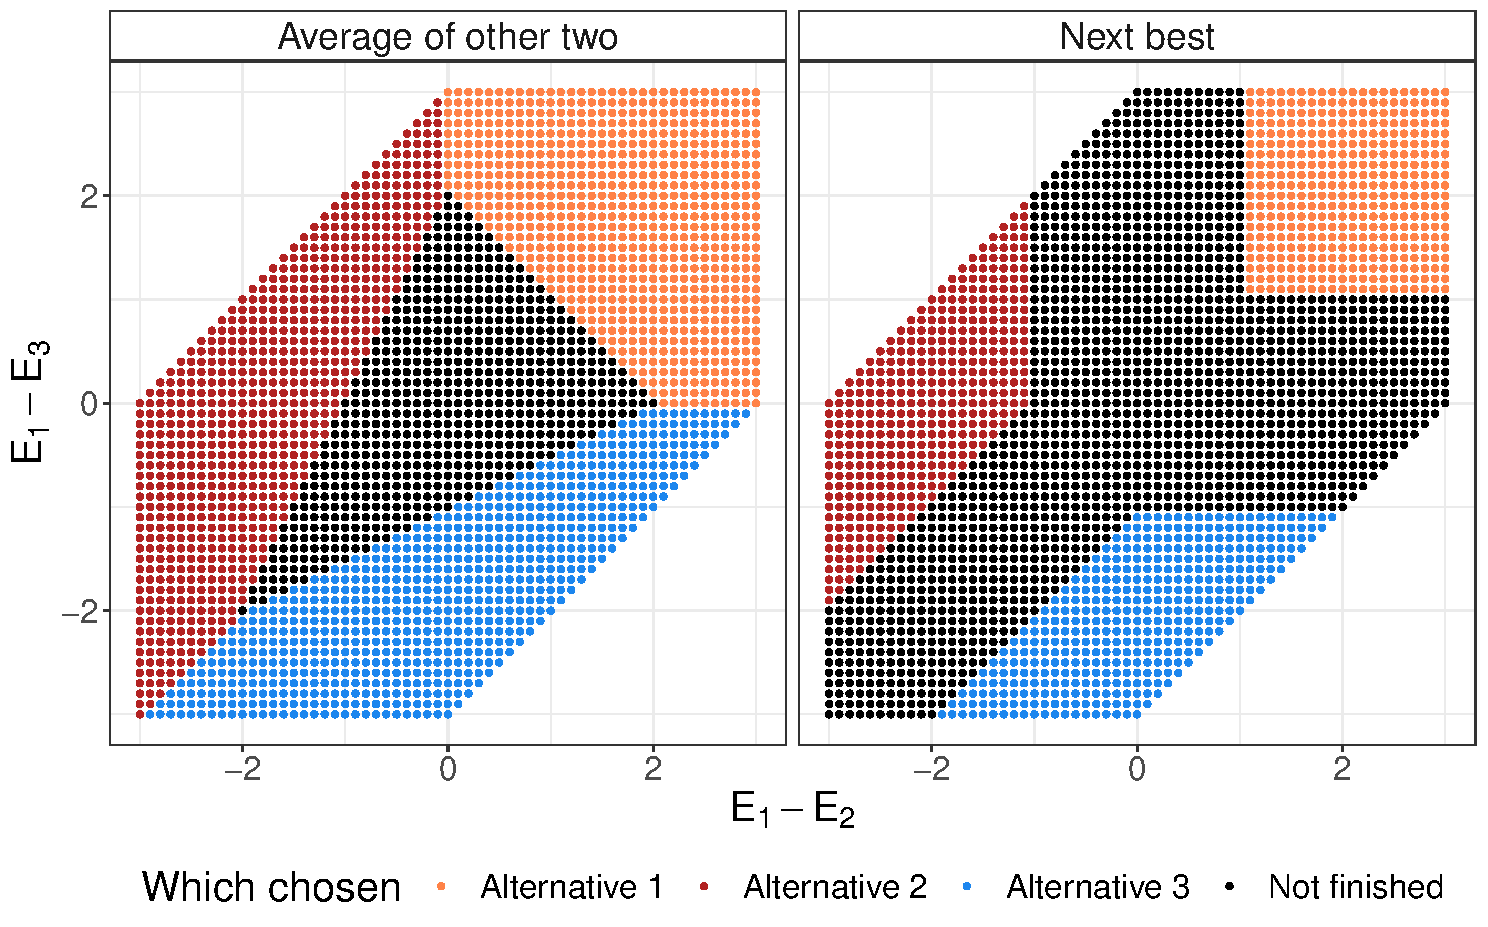
\includegraphics[width=1\textwidth]{rulesfinished.pdf}
\label{fig:rulesfinished}
\end{figure}

As mentioned, we wished to calculate the probability distribution over the relative evidence states $E_{1}-E_{2}$ and $E_{1}-E_{3}$ (each of which is represented by a dot on Figure \ref{fig:rulesfinished}) for a given parameter set and time step. Assuming that each step in the process can be described by a two-dimensional vector with components
\begin{equation}
\begin{array}{l}
\displaystyle x = E_{1}-E_{2} = d(\theta_{t}r^1-\theta_{t}r^2) + (\varepsilon_{t}^{1}-\varepsilon_{t}^{2})\\
\displaystyle y = E_{1}-E_{3} = d(\theta_{t}r^1-\theta_{t}r^3) + (\varepsilon_{t}^{1}-\varepsilon_{t}^{3}),\\
\end{array} 
\label{eq:axes1}
\end{equation}

the covariance matrix between the two axes is

\begin{equation}
\begin{array}{l}
COV = \begin{bmatrix}
       2\sigma^2 & \sigma^2 \\[0.3em]
       \sigma^2 & 2\sigma^2 \\[0.3em]
     \end{bmatrix}
\end{array} 
\label{eq:covariance}
\end{equation}

This covariance matrix is not diagonal, because the axes are correlated (due to the shared component $\varepsilon_{t}^{1}$ in the relative evidence states), which, when modelling the process, results in an ellipse whose axes are not parallel to the coordinate axes (see the left panel on Figure \ref{fig:rotate}). Such correlation between the two relative evidence states would lead to biased probability estimates. To address this issue and eliminate the correlation between the axes, we can place them at a more convenient position, by rotating both axes by an angle $\alpha$ (as demonstrated in the right panel of Figure \ref{fig:rotate}). 
%This could be improved

\begin{figure}[htb!]
\captionsetup{justification=centering}
\centering
\caption{Demonstration of the correlation problem. The left panel shows the original axes, whereas the right panel shows the rotated axes with no correlation.}
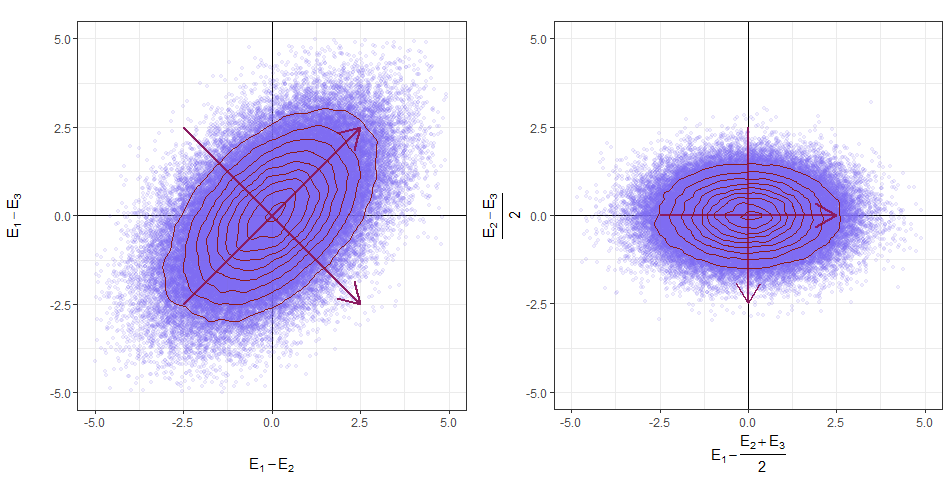
\includegraphics[width=1\textwidth]{rotate.pdf}
\label{fig:rotate}
\end{figure}
 

Assuming $x'$ and $y'$ are the respective rotated versions of $x$ and $y$, they can be characterised as
\begin{equation}
\begin{array}{l}
\displaystyle x' = x cos(\alpha) + y sin(\alpha)\\
\displaystyle y' = -x sin(\alpha) + y cos(\alpha).\\
\end{array} 
\label{eq:axes2}
\end{equation}

The next step was to calculate the value of $\alpha$ that results in a diagonal covariance matrix between $x'$ and $y'$ (corresponding to no correlation between the two axes). One solution for this system is given by $cos(\alpha) = sin(\alpha)$, or $\alpha = 45\degree$. Expressed in terms of our original relative evidence states, a $45\degree$ degree anti-clockwise rotation results in the new axes defined as

\begin{equation}
\begin{array}{l}
\displaystyle x' = E_{1}-\frac{E_{2}+E_{3}}{2}\\
\displaystyle y' = \frac{E_{2}-E_{3}}{2}.\\
\end{array} 
\label{eq:axes1}
\end{equation}
 
As the right panel in Figure \ref{fig:rotate} demonstrates, this results in an ellipse whose axes are now parallel to the coordinate axes. In this transformed coordinate system, we can characterise the decision process as a multivariate normal distribution whose movement along the relative evidence bins is governed by the model parameters. To save computation time, the possible evidence states were approximated by bins (the x evidence space spanned from -2.5 to 1.5 with spacing 0.1 in 41 bins, whereas the y evidence space spanned from -1.5 to 1.5 with spacing 0.1 in 31 bins, resulting in $31x41 = 1271$ bins). Then, using the preference ratings $r$, the penalty on the unattended item $\theta$, the speed of integration $d$, and the variance of the normal distribution $\sigma$, we can define three $1271x1271$ matrices (corresponding to fixating on each of the three choice items) that represents the probability of transition from and to each of the new relative evidence states. 

In each trial, at time step 0, the process is in the bin defined by $x = 0$ and $y = 0$, with probability density 1. Knowing which item is fixated first, we can calculate the probability distribution over the relative evidence states at time step 1, by multiplying the current probability distribution with the corresponding transition matrix. As a result of this process, with each time step before the final one, the probability mass diffuses and moves, governed by the drift rate, and any probability mass outside the triangle (corresponding to evidence states where the process has finished) gets reset to 0. This way, we can calculate the exact probability that the process finishes in the correct time bin (given by the choice data). In the last time bin, we can simply sum the probabilities over the relative evidence states that correspond to the eventually chosen item. The upper panel in Figure \ref{fig:process} illustrates the movement of the probability mass over time, whereas the lower panel shows the summed probabilities after each time step. To make sure that this estimation method is completely free of stochasticity, we used a deterministic fixation pattern, based on which item was fixated first in the 200 ms bin. 

Once we were able to calculate the choice probabilities using this method, we again started off with a grid search to find the best fitting parameters for each participant and subjective value transformation rule. We used the following $3x3x3=27$ parameter grid: $\theta=\{0.33, 0.67, 1\}$, $\sigma=\{0.1, 0.55, 1\}$, \textit{d}=$\{0.1, 0.55, 1\}$ in running the Nelder-Mead optimization algorithm. We used a smaller grid, because there is no stochasticity in this method, but it is also computationally more intensive to calculate (calculating the likelihood for one participant takes 13 times longer compared to the simulation approach). For the same reason, we only ran the Nelder-Mead process once more after the grid search with a maximum iteration number of 100.  


\newcounter{savepage}
\cleardoublepage
\setcounter{savepage}{\arabic{page}}
\newgeometry{left=1cm,bottom=1cm, right = 1cm, top = 1cm}
\begin{landscape}
\pagenumbering{gobble}
\begin{figure}
\captionsetup{justification=centering}
\caption{Illustration of the diffusion process over 8 time steps with attention pattern $1, 1, 2, 2, 2, 3, 3, 3$; $\sigma = 0.3$; $\theta = 0.67$; $d = 1$, $r = 0.5, 0.5, 0.5$}
\centering
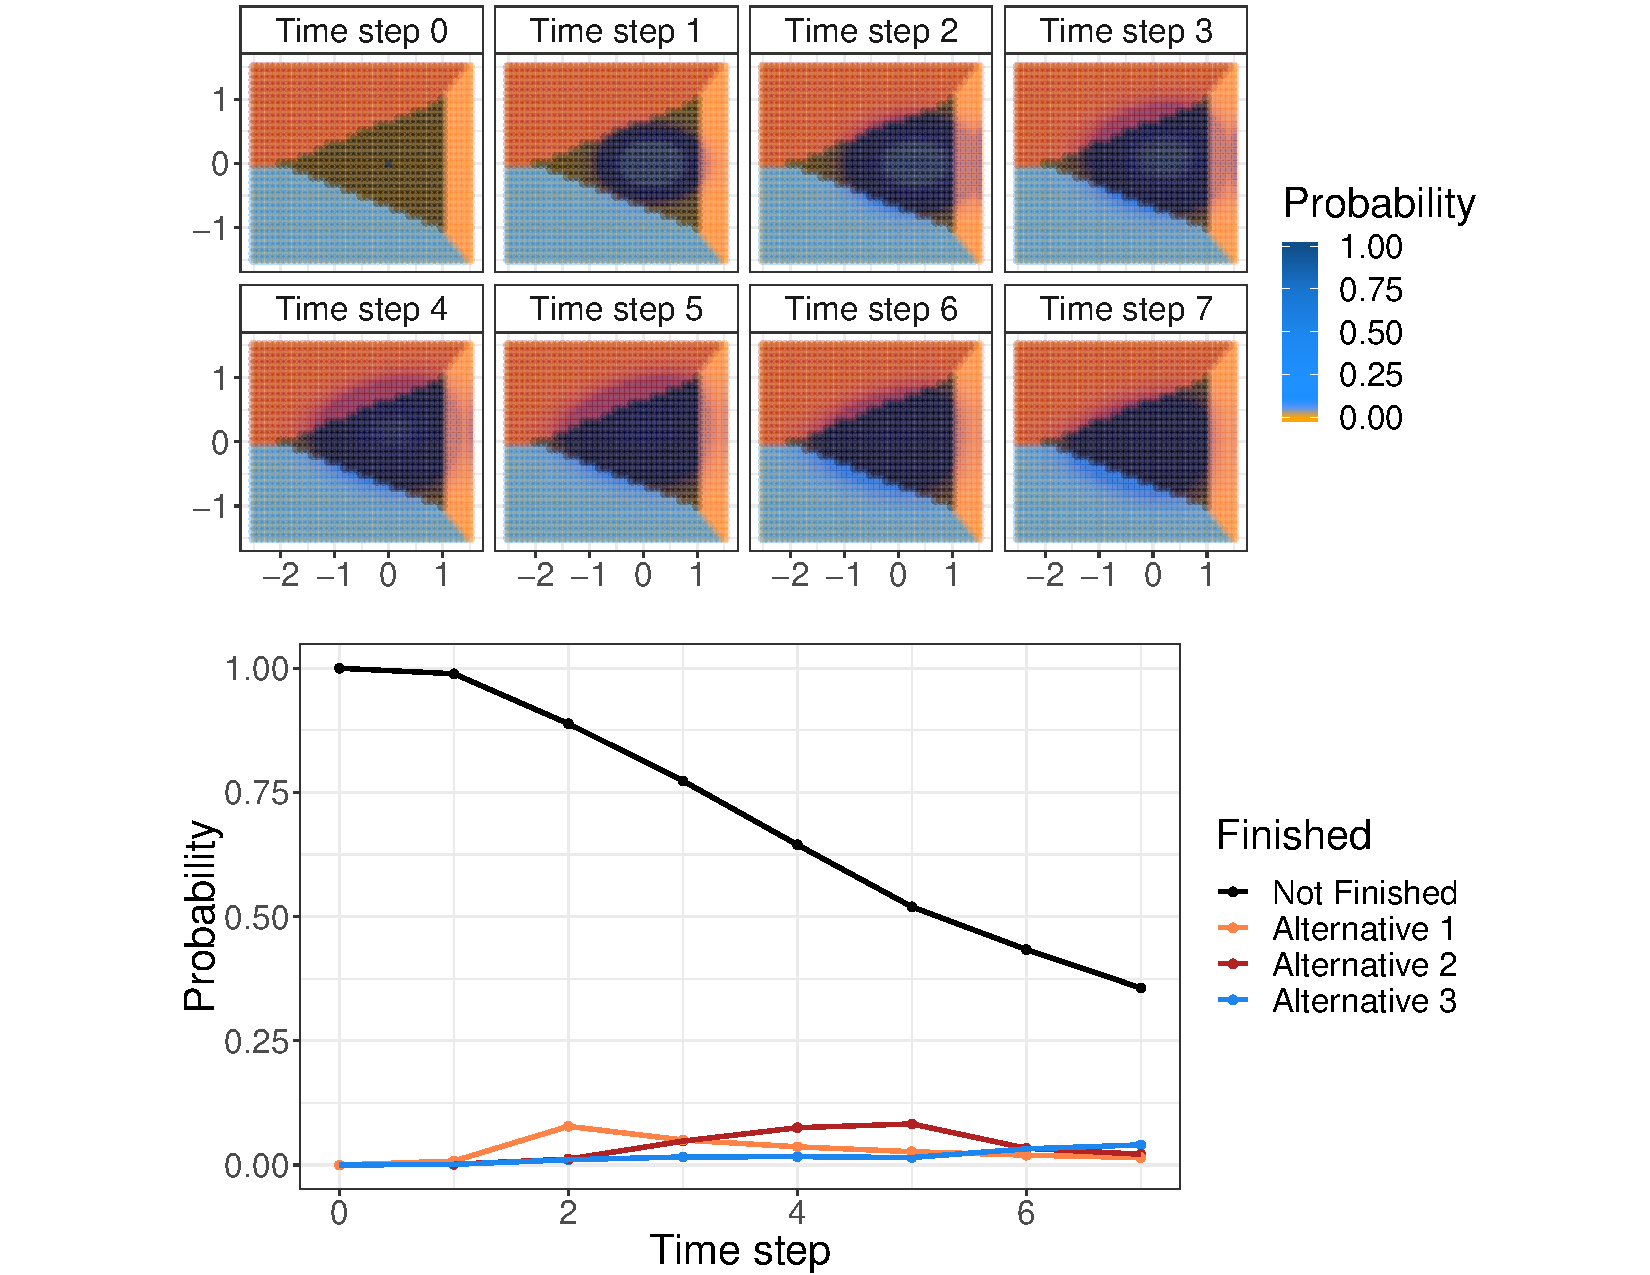
\includegraphics[width=1\textwidth]{process.pdf}
\label{fig:process}
\end{figure}
\end{landscape}
\restoregeometry
\cleardoublepage
\pagenumbering{arabic}
\setcounter{page}{\thesavepage} 
 

\subsection{Results}

The model fitting process resulted in $50x4=200$ likelihoods for each of the two methods, for each participant and value transformation rule. We wished to determine which value transformation rule produces the highest likelihood for each participant and method. Since the fitted models have the same number of parameters and are calculated on the same set of data, the likelihoods are directly comparable. Table \ref{table:chap1res} shows the result of this comparison by estimation method.
 
 
\begin{table}[ht]
\caption{Best fitting model for each participant by estimation method.}
\centering
\begin{tabular}{ccccc}   

\toprule Approach  & Global Max    & Local Max & Rank & Range \\ 
\midrule Simulations  &  29 (58\%) & 11 (22\%)  & 4 (8\%)   & 6 (12\%) \\
       Probability Distribution & 29 (58\%)  &    10 (20\%)    & 6 (12\%)   & 5  (10\%)  \\
\bottomrule 
\end{tabular}
\label{table:chap1res}
\end{table}

The two estimation approaches have yielded very similar results. For the majority of participants (58\%), the global maximum rule provided the best fit, regardless of the estimation approach. This is followed by the local maximum rule, which provided the best fit for 22-20\% of the participants. The range and rank rules proved to be the best fitting model for only about 10\% of participants. Overall, these results point to a mechanism where subjective valuation mostly depends on the absolute value of the options, and, albeit to a lesser extent, is also affected by the relative magnitude of the options (compared to the maximum value on the current trial). In addition, the almost identical results from the two estimation approaches underline the robustness of the findings, and alleviates concerns about the reliability of the simulations approach.

 
 
\section{Experiment 2}

In Experiment 2, we were still interested in testing the explanatory power of the four value transformation rules using the choice set manipulations, but we used a fundamentally different stimuli and estimation approach.

Experiment 2 had several rationales. First and foremost, comparing the results from a qualitative comparison of choice probabilities with the results from a model fitting approach allows us to gain a deeper understanding of the relative explanatory power of each value transformation rule. While we have some choice data on the seven relevant choice sets from Experiment 1, due to the error in the experimental procedure, it is not enough to conduct a test with appropriate statistical power. Second, it can be argued that the preference ratings participants gave in the first part of Experiment 1 are already context-dependent, since the movies are evaluated with respect to each other in the ratings task, which could affect our results. Finally, since the movie stimuli is somewhat complex in the sense that there are a range of factors we could not control for (e.g. visual saliency, mnemonic processes the stimuli can induce), it seems appropriate to repeat the experiment with a simpler, and more neutral stimuli. 

\subsection{Method}

We recruited 130 participants through the University of Warwick's Research Participation System. On each trial, participants were presented with a trinary set of rapidly changing sequences of numbers (first used in \citeauthor{Tsetsos2012a}) and were asked to pick the sequence with the highest average of numbers by pressing the corresponding keyboard key (left, down, right arrow). The numbers were updated every 210-250 ms. To familiarise participants with the task, the experiment began with three practice trials, where feedback were given on which sequence they chose. After the practice trials, there were 140 trials to be completed in two blocks. Participants could take a break for as long as they wished between the two blocks and they were paid £5.00 for taking part in the experiment. Figure \ref{experi2_numbers} shows one trial from this experiment. The experiment on average took about 15 minutes to complete. Ethical approval was obtained from the Department of Psychology, University of Warwick.

\begin{figure}
\captionsetup{justification=centering}
\centering
\caption{Example trial from Experiment 2.}
\includegraphics[width=0.7\textwidth]{experi2.png}
\label{fig:experi2_numbers}
\end{figure}

\subsection{Stimuli}

Numbers for each presented sequence were derived from a truncated normal distribution with a standard deviation of 18, and a mean that was calculated from a monotonic transformation of the ratings from Experiment 1. Specifically, we multiplied each number by ten and then added ten to them, so a trial with values 1,2,4 in Experiment 1 corresponded to a trial with means 20, 30, 50 in Experiment 2. The distribution was truncated to only include numbers between 0 and 99. We chose to work with the two-digit equivalents of the values from Experiment 1 to increase the range of numbers that could be sampled, and the constant was added to shift the lower end of the value distributions away from 0. When a number below 10 was sampled, it was displayed as a two-digit number with 0 as the first digit. 


\subsection{Results}

For a qualitative test of the four value transformation rules, for each choice set manipulation, we compared the resulting choice proportions from both experiments with predictions from simulating out the ddm. These simulations focused only on the eventually chosen item, and did not take into account the RTs. Although the qualitative patterns of predicted choice proportions are largely insensitive to the exact parameter values, for the sake of comparability, we decided to use the same parameter pair ($\sigma$ and \textit{d}) in all simulations. This parameter pair was derived in the following way.

Using data from Experiment 1, our main was to select the parameter pair that provided the best fit across all four value transformation rules on average. First, using a $5x5=25$ grid space with $d=\{0.01, 0.03, 0.1, 0.32, 1\}$ and $\sigma=\{0.01, 0.03, 0.1, 0.32, 1\}$,  we calculated the difference between the predicted and actual choice probabilities for each parameter pair and value transformation rule. We simulated out the ddm 100,000 times to obtain the predicted probabilities. This allowed us to rank each of the 25 parameter pairs for each value transformation rule based on how well it fits the actual data (for each rule, the parameter pair that produced the smallest difference between predicted and actual probabilities was allocated a rank of 1, while the pair that produced the highest difference receved a rank of 25). Then, using the parameter pair that had the smallest sum of ranks across the four value transformation rules, we started a Nelder-Mead optimisation process that aimed to minimise the average probability difference across all rules. We once more restarted the Nelder-Mead process using the previous parameter results, which finally produced the parameter pair $d=0.012$ and $\sigma=0.0761$.

Figures \ref{fig:addconstant_all}-\ref{fig:multiply_all} show the results from this qualitative comparison. In these figures, the four panels to the left correspond to the choice proportion predictions from the ddm simulations, while the two panels on the right show the resulting choice proportions from the two experiments and their associated 95\% CIs. All model predictions are based on 100,000 simulations. The difference in the precision of the estimates from the two experiments reflects the differences in the amount of choice data for the relevant choice sets.  

\textbf{Adding a constant.} Figure \ref{fig:addconstant_all} shows the effect of adding a constant. Unfortunately, the wide confidence intervals around the choice proportions from Experiment 1 do not allow us to see any clear patterns, but the results from Experiment 2 are broadly in line with the predictions from the local maximum rule. In summary, the results from adding a constant lend partial support to the local maximum rule.  


\begin{figure}[!htb]
\captionsetup{justification=centering}
\centering
\caption{Choice set manipulation adding a constant}
\includegraphics[width=0.9\textwidth]{exp1_addconstres.pdf}
\label{fig:addconstant_all}
\end{figure}

\textbf{Multiplying by a constant.} Figure \ref{fig:multiply_all} shows the effect of multiplying each value by a constant, where only the global maximum rule predicts a change in the choice proportions. Specifically, it predicts that the best option will benefit from adding a constant to each value. The results from both experiments are in line with these predictions, strongly supporting the global maximum rule.

\begin{figure}[!htb]
\captionsetup{justification=centering}
\centering
\caption{Choice set manipulation multiplication by constant}
\includegraphics[width=0.9\textwidth]{exp1_multiplytres.pdf}
\label{fig:multiply_all}
\end{figure}

\textbf{Distant vs close second.} Figure \ref{fig:distclose2nd_all} shows the results from the close versus distant second choice set manipulation. Only the rank rule does not predict any change in the choice proportions, and we chose this manipulation because it allows us to evaluate the explanatory power of the rank rule. Results from the two experiments show that there is a substantial change in the choice proportions, as the middle item becomes relatively more attractive compared to the best item, which was predicted by all the other value transformation rules. Therefore, the distant versus close second choice manipulation rules provides strong evidence against the rank rule. 


\begin{figure}[!htb]
\captionsetup{justification=centering}
\centering
\caption{Choice set manipulation close versus distant middle}
\includegraphics[width=0.9\textwidth]{exp1_distclosesecres.pdf}
\label{fig:distclose2nd_all}
\end{figure}

\textbf{Distant vs close third.} Finally, Figure \ref{fig:closedist3rd_all} shows the results from the close versus distant third choice set manipulation. The predictions of the value transformation rules differ significantly, the two maximum rules predicting that the worst option will benefit at the expense of the other two, the range rule predicting that the middle item will become relatively less attractive compared to the best due to the increased proximity of the worst item and the decrease in the range of values. The rank rule does not predict any change.  While the results from Experiment 2 unequivocally support the predictions of the two maximum rules, the results form Experiment 1 are more mixed (although we can detect a clear increase in the choice proportion of the  middle item). Therefore, the close versus distant third offers support for the two maximum rules.

\begin{figure}[!htb]
\captionsetup{justification=centering}
\centering
\caption{Choice set manipulation close versus distant third}
\includegraphics[width=0.9\textwidth]{exp1_distclosethirdres.pdf}
\label{fig:closedist3rd_all}
\end{figure}


To summarize, the results from the qualitative comparisons suggest that the two maximum normalisation rules had the highest explanatory power. More specifically, albeit to varying degrees, but both rules predicted the effect of three out of the four choice set manipulations, the range rule successfully predicted one, and the rank rule did not predict the effect of any of the choice set manipulations.

This can be contrasted with the results from the model fitting approach, which indicated that the global maximum rule has the highest explanatory power by far. In line with this, multiplication by a constant, which was only correctly predicted by the global maximum rule, resulted in the largest difference between choice proportions in Experiment 1.


In addition, interestingly, even though the two experiments involved fundamentally different stimuli (complex versus perceptual), the effects of the choice set manipulations on the choice proportions turned out to be rather similar. Unfortunately, a strict comparison of the two datasets is hindered by the relatively small sample size of Experiment 1. Nevertheless, the results lend some support to the idea that there exists a common valuation mechanism across a range of stimuli domains.



\newpage

\section{Discussion}

In this research project, our aim was to conduct a comprehensive evaluation of the relative explanatory power of four different forms of context-dependency. To compare four value transformation rules, each of which captures a different form of context-dependent valuation, we used a popular cognitive model, the ddm and its extension, the aDDM, to derive predictions about choice behaviour in two choice experiments with trinary choice sets, one with complex stimuli (movie posters), and another one with a perceptual task.

Two fundamentally different approaches, a quantitative approach that entailed fitting the aDDM to choice and eye-tracking data from Experiment 1, and a qualitative approach, involving the inspection of resulting choice proportions from both experiments were used for the comparison. The results from the two comparison methods were broadly in line, both supporting the view that while subjective valuation mostly reflects the absolute magnitude of the options under consideration, to a lesser extent, it is also affected by the relative value of the options (within the local context).

These findings are consistent with insights from research investigating the neural correlates of value-based decision making. Results from numerous neuroeconomic studies strongly support the view that the orbifrontal cortex (OFC) is the brain region where subjective value encoding takes place in economic choices (for a review see \citeNP{Padoa-Schioppa2017}). Moreover, it has been suggested that there is a group of neurons in the OFC with two fundamental properties that are likely to be directly responsible for simultaneous absolute and relative value sensitivity in economic valuation.

First, \citeA{Padoa-Schioppa2008} have shown that such neurons exhibit menu invariance, meaning that the value assigned to each option under consideration is independent from the value of the rest of the available alternatives, reflecting the absolute value of the option (global maximum in our experiments). Menu invariance gives rise to preference transitivity, ensuring that preferences are stable across the wide range of contexts the decision maker might encounter. Second, there is ample evidence that neuronal firing rates adapt to the range of available values (e.g., \citeNP{Padoa-Schioppa2009}; \citeNP{Louie2013}). Such adaptation is widespread in sensory systems, and is a natural consequence of biophysical constraints. Interestingly, although the most commonly proposed form of adaptation in the neuroeconomic literature is is range adaptation (e.g., \citeNP{Soltani2012}), our data suggests that normalising by the maximum on the current trials fares better at predicting choice.

There exist other ways to approach this question within the sequential sampling framework. In particular, instead of changing the input values of the accumulation equation, we could have focused on how these values are integrated and incorporated into the accumulation process. This is what \citeA{Teodorescu2016} did in a somewhat similar investigation to ours. Specifically, they contrasted relative and absolute evidence processing in a sequential sampling framework by comparing an independent race model (capturing absolute value processing, where the input is the absolute value of the options), with a ddm model (where differences of input values govern the accumulation process). 

In their experiment, participants were instructed to choose the brighter out of two, fluctuating grey patches, with a fixed mean brightness. They focused on two manipulations: in an additive-boost condition, they added the same constant to both means, preserving the difference between the two mean brightness, whereas in the multiplicative-boost condition, they multiplied both means by the same constant, preserving the ratio of the two means. These conditions are direct equivalents to our add a constant, and multiply by a constant choice set manipulations.

Interestingly, they found that no "pure" (either entirely absolute or relative) accumulation model could account for the data, and thus they propose two distinct types  of models that can account for this pattern: a ddm model where the noise in the process is a function of the intensity of the inputs, and a leaky competing accumulator model (LCA; \citeNP{Usher2001}), where simultaneous absolute and relative value sensitivity is a product of lateral inhibition. 

things to mention :

1) no mistake would have been better

2) Another approach could have been to test the explanatory power of these value transformation rules by manipulating the temporal order of the values

\bibliographystyle{apacite}

\newpage

\bibliography{refs}

\end{document}